% circuit-sim-lab-report — report.tex
% Course 0714-EEE-2102, Circuit Simulation Laboratory
% Experiment 4 — full-wave bridge rectifier with and without filter capacitor
%
% Compile (twice, from Lab_report_latex/):
%   env pdflatex -interaction=nonstopmode report.tex

\documentclass[12pt,a4paper]{article}

% ----- Page geometry: A4, 1 inch margins all sides -----
\usepackage[margin=1in]{geometry}

% ----- Times New Roman (text + math) -----
\usepackage{newtxtext,newtxmath}

% ----- Spacing: 1.5 line spacing, 6 pt paragraph spacing -----
\usepackage{setspace}
\onehalfspacing
\usepackage{parskip}          % paragraph gaps instead of indents
\setlength{\parskip}{6pt plus 1pt}

% ----- Math, SI units -----
\usepackage{amsmath}
\usepackage{siunitx}

% ----- Graphics, tables, captions, floats -----
\usepackage{graphicx}
\usepackage{booktabs}
\usepackage[american]{circuitikz}
\usetikzlibrary{arrows.meta,calc}

\usepackage{caption}
\usepackage{float}
\usepackage{array}
\usepackage[table]{xcolor} % row shading for Word-style table headers
% waveform-figure colours (theory section)
\definecolor{wvpos}{RGB}{250,226,166}
\definecolor{wvneg}{RGB}{214,204,236}
\definecolor{wvout}{RGB}{176,214,160}
\definecolor{wvon}{RGB}{36,110,60}
\definecolor{wvoff}{RGB}{110,70,150}
\definecolor{wvvd}{RGB}{190,40,60}
\graphicspath{{../graphs/}{./figures/}}

% ----- Lists: compact, guide-style itemization -----
\usepackage{enumitem}
\setlist{nosep, leftmargin=2em, label=\textbullet}

% ----- Front matter and PDF output -----
\usepackage{pdfpages}
\usepackage[hidelinks]{hyperref}

% ----- Headings: bold, left-aligned, 14/15 pt -----
\usepackage{titlesec}
\titleformat{\section}
{\normalfont\Large\bfseries}{\thesection}{0.8em}{}
\titleformat{\subsection}
{\normalfont\large\bfseries}{\thesubsection}{0.8em}{}
\titlespacing*{\section}{0pt}{*3}{*2}
\titlespacing*{\subsection}{0pt}{*2.5}{*1.5}

% ----- Captions: centered, 11 pt, figures below / tables above -----
\captionsetup{font=small, labelfont=bf, justification=centering}
\captionsetup[table]{position=above, skip=4pt, labelfont=normalfont}
\captionsetup[figure]{position=below, skip=4pt, labelfont=normalfont}

% ----- Page number: bottom-center -----
\usepackage{fancyhdr}
\pagestyle{fancy}
\fancyhf{}
%\fancyfoot[C]{\thepage}
\renewcommand{\headrulewidth}{0pt}

% ----- Experiment number: sections then number 4.1-4.9 -----
\newcommand{\expnumber}{4}
\renewcommand{\thesection}{\expnumber.\arabic{section}}
\begin{document}
	
	\section*{4.4 PSpice Circuit Diagrams}
	\setcounter{figure}{4}   % Next figure will be Figure 6
	\begin{figure}[H]
		\centering
		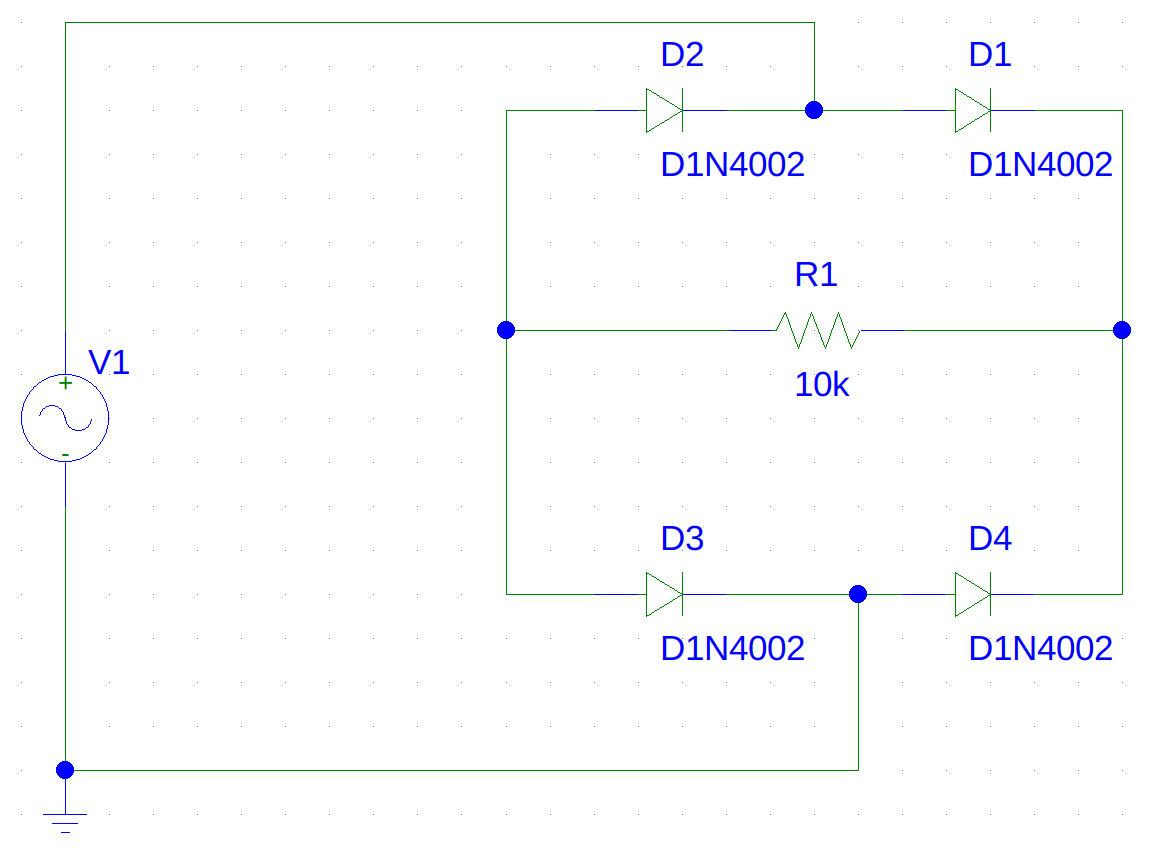
\includegraphics[width=0.8\textwidth]{schematic_no_filter.png}
		\caption{PSpice schematic of the full-wave bridge rectifier without
			filter capacitor ($R_1 = \SI{10}{\kilo\ohm}$,
			$V_{\mathrm{in}} = \SI{100}{\volt}$ amplitude at \SI{50}{\hertz})}
		\label{fig:sch1}
		
	\end{figure}
	
	
	\begin{figure}[H]
		\centering
		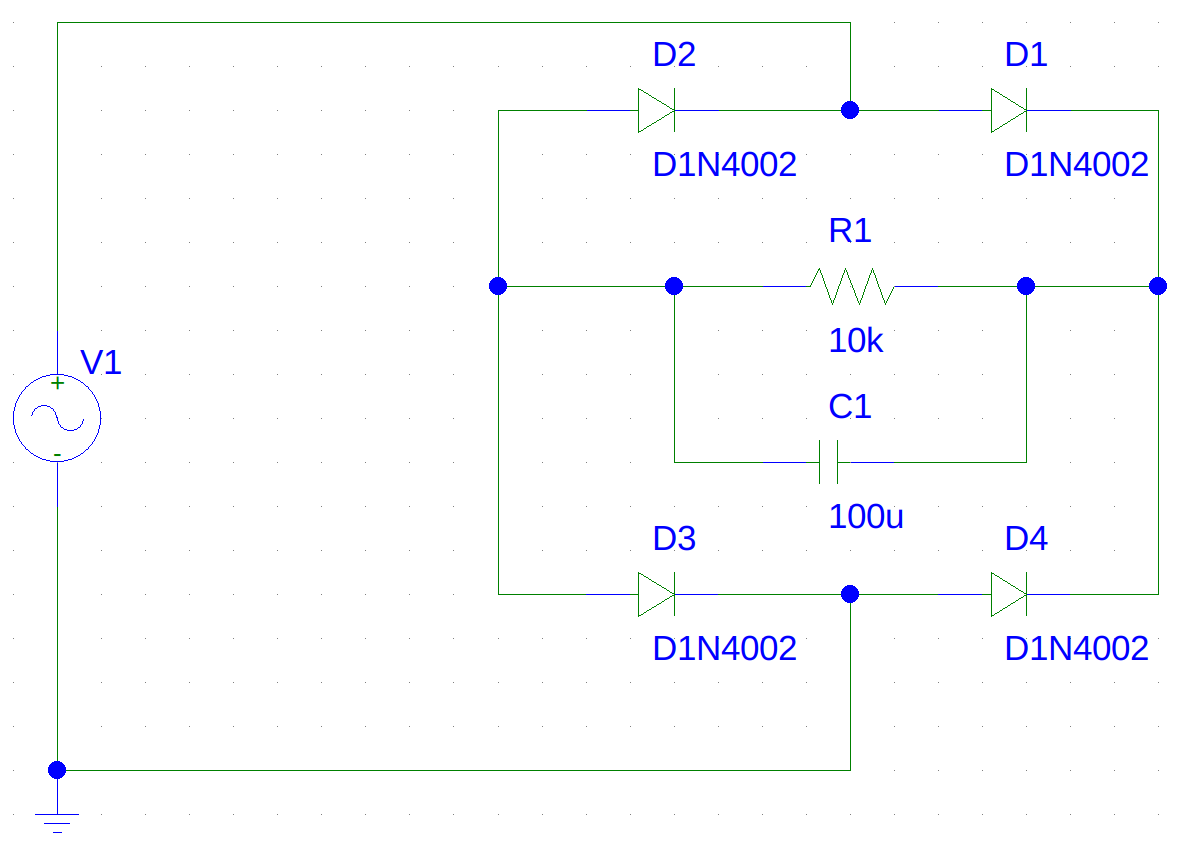
\includegraphics[width=0.8\textwidth]{schematic_with_capacitor.png}
		\caption{PSpice schematic of the full-wave bridge rectifier with
			filter capacitor ($C_1 = \SI{100}{\micro\farad}$ in parallel with
			$R_1 = \SI{10}{\kilo\ohm}$)}
		\label{fig:sch2}
	\end{figure}
	
	\begin{figure}[H]
		\centering
		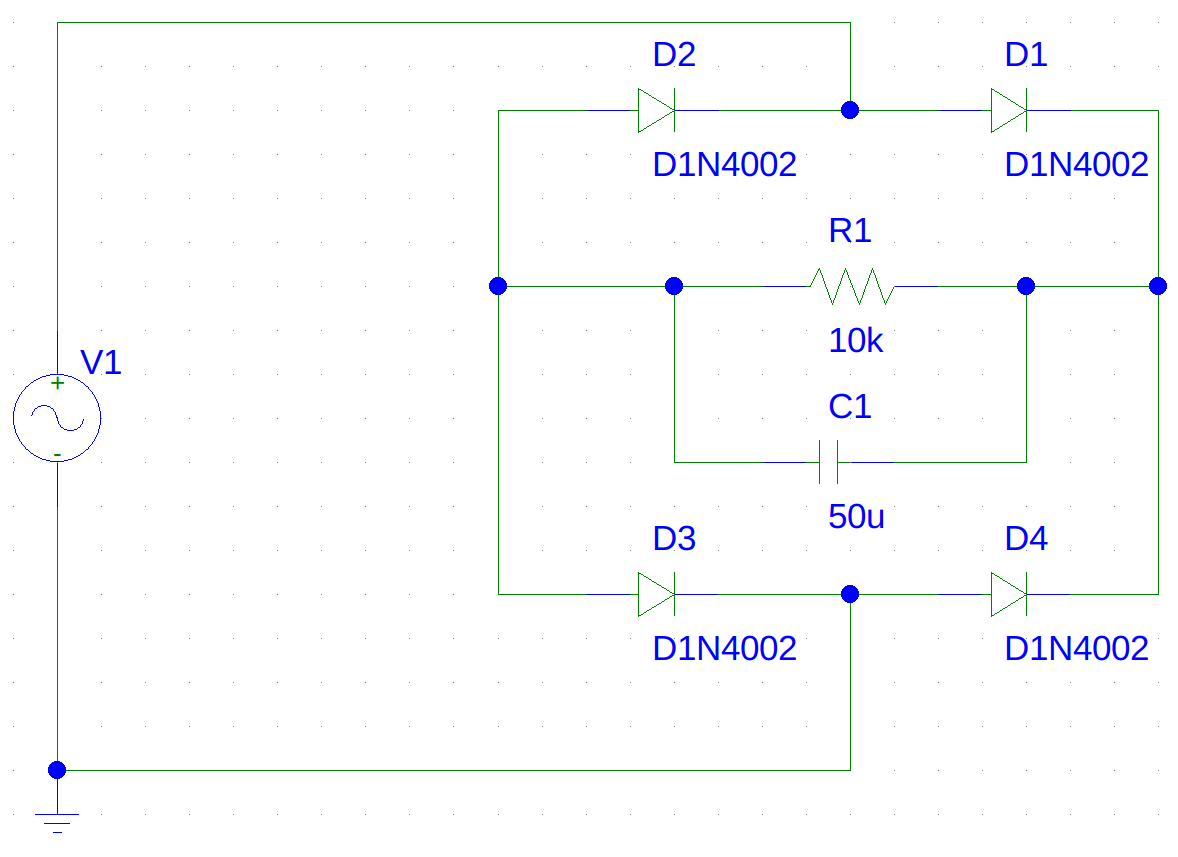
\includegraphics[width=0.8\textwidth]{schematic_with_capacitor_changed.png}
		\caption{PSpice schematic of the modified bridge rectifier (task 4,
			filter capacitor changed to $C_1 = \SI{50}{\micro\farad}$)}
		\label{fig:sch3}
	\end{figure}
	
	\newpage
	
	\section*{4.7 Result Analysis}
	% =====================================================================
	\subsection*{4.7.1 Simulated waveforms}
	
	\setcounter{figure}{7}   % Next figure will be Figure 6
	
	\begin{figure}[H]
		\centering
		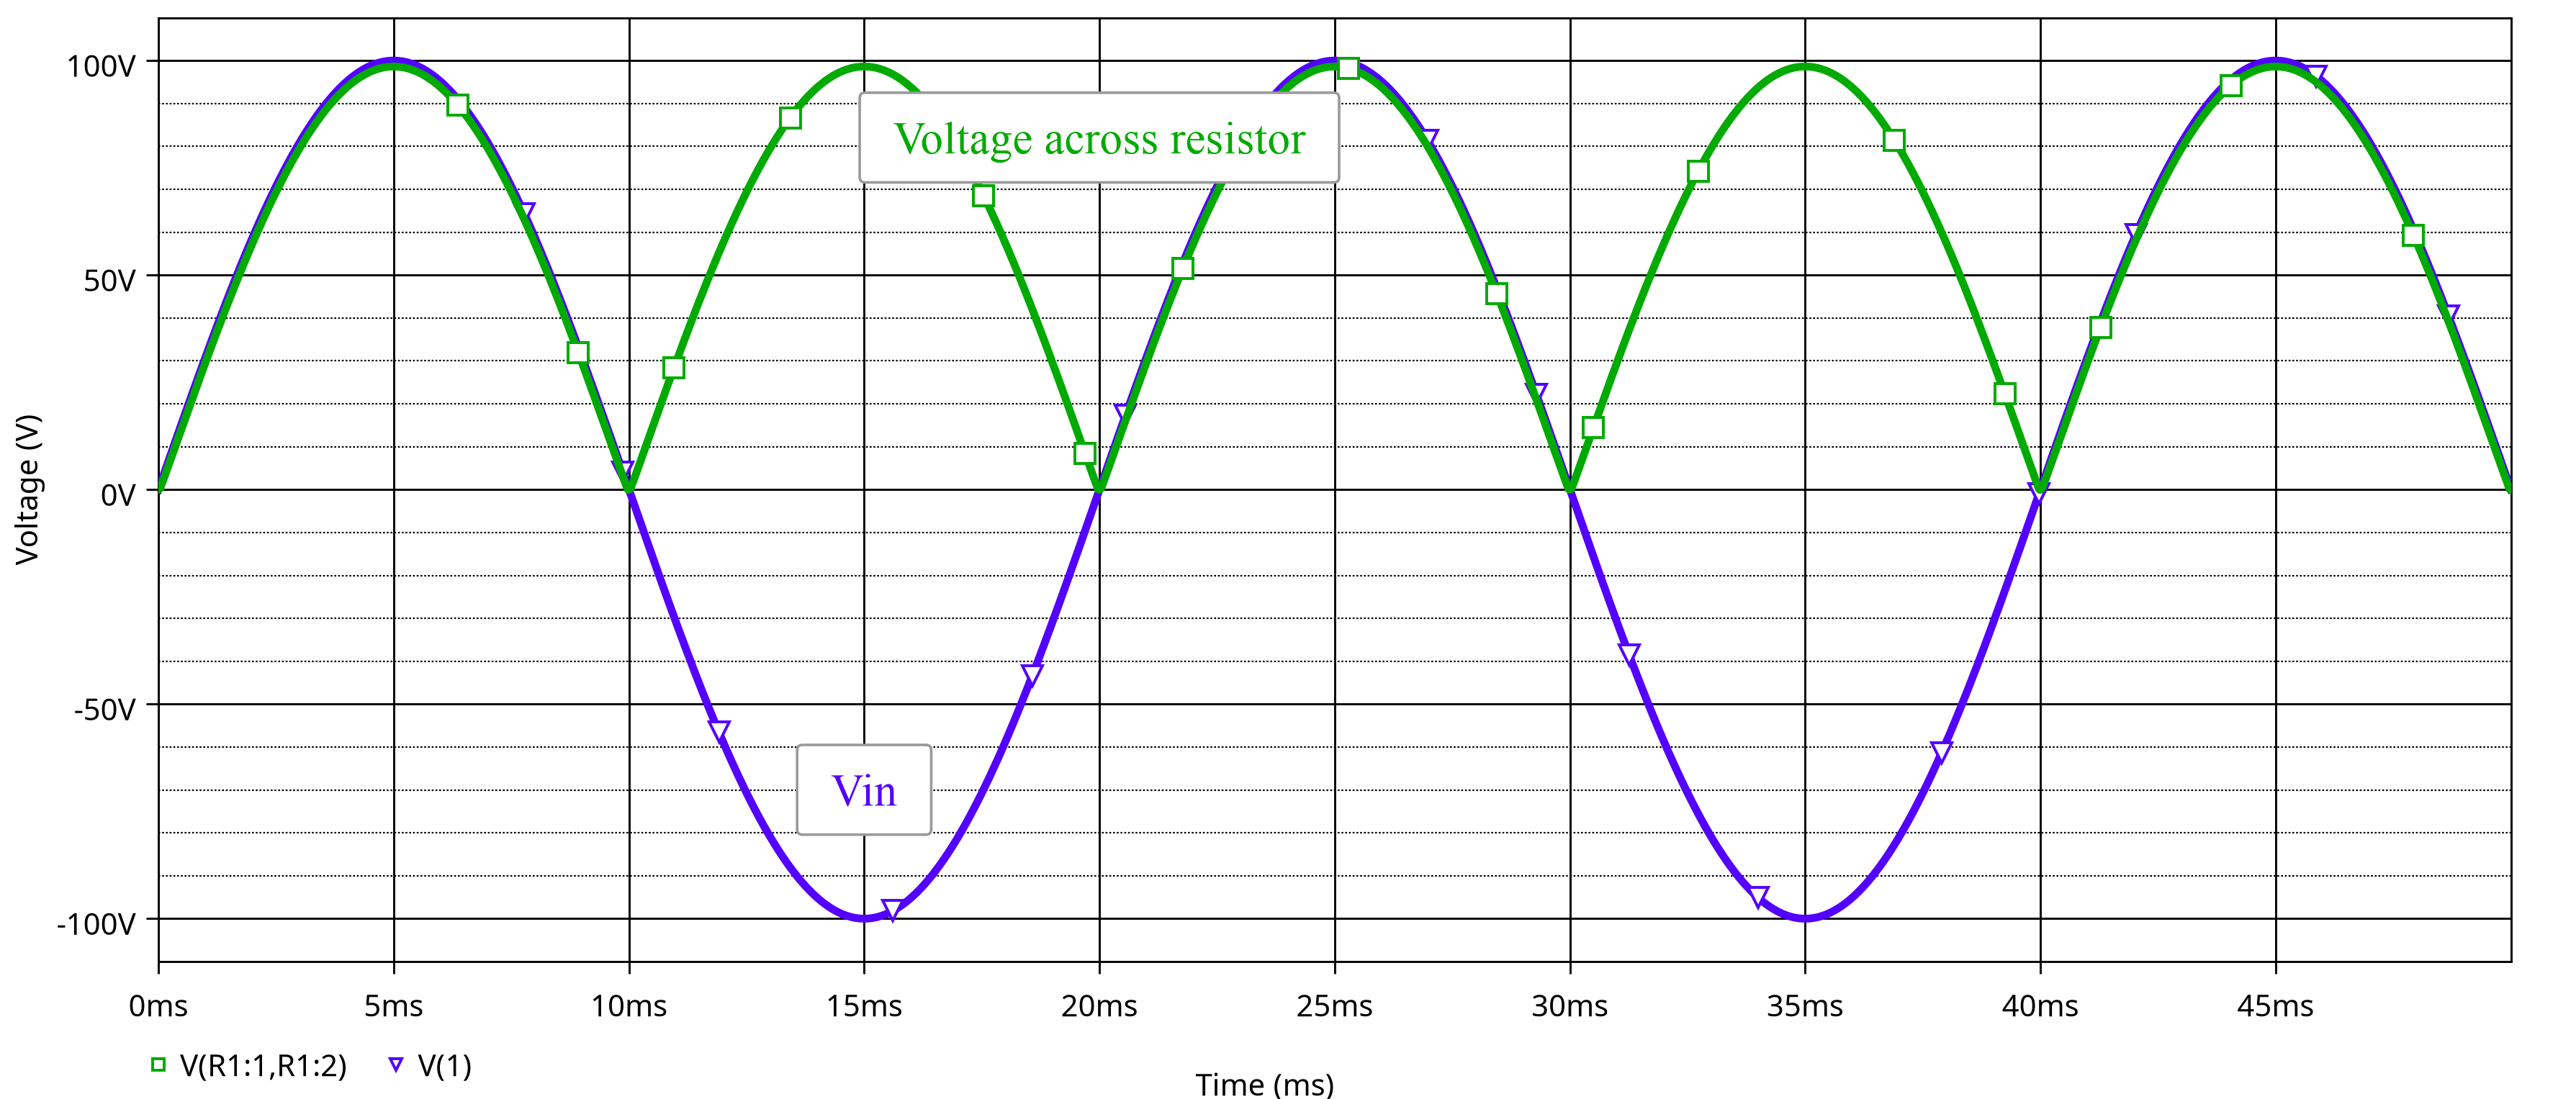
\includegraphics[width=0.8\textwidth]{full_bridge.png}
		\caption{PSpice output: input and load-voltage waveforms of the
			bridge rectifier without filter capacitor}
		\label{fig:wave1}
	\end{figure}
	
	\begin{figure}[H]
		\centering
		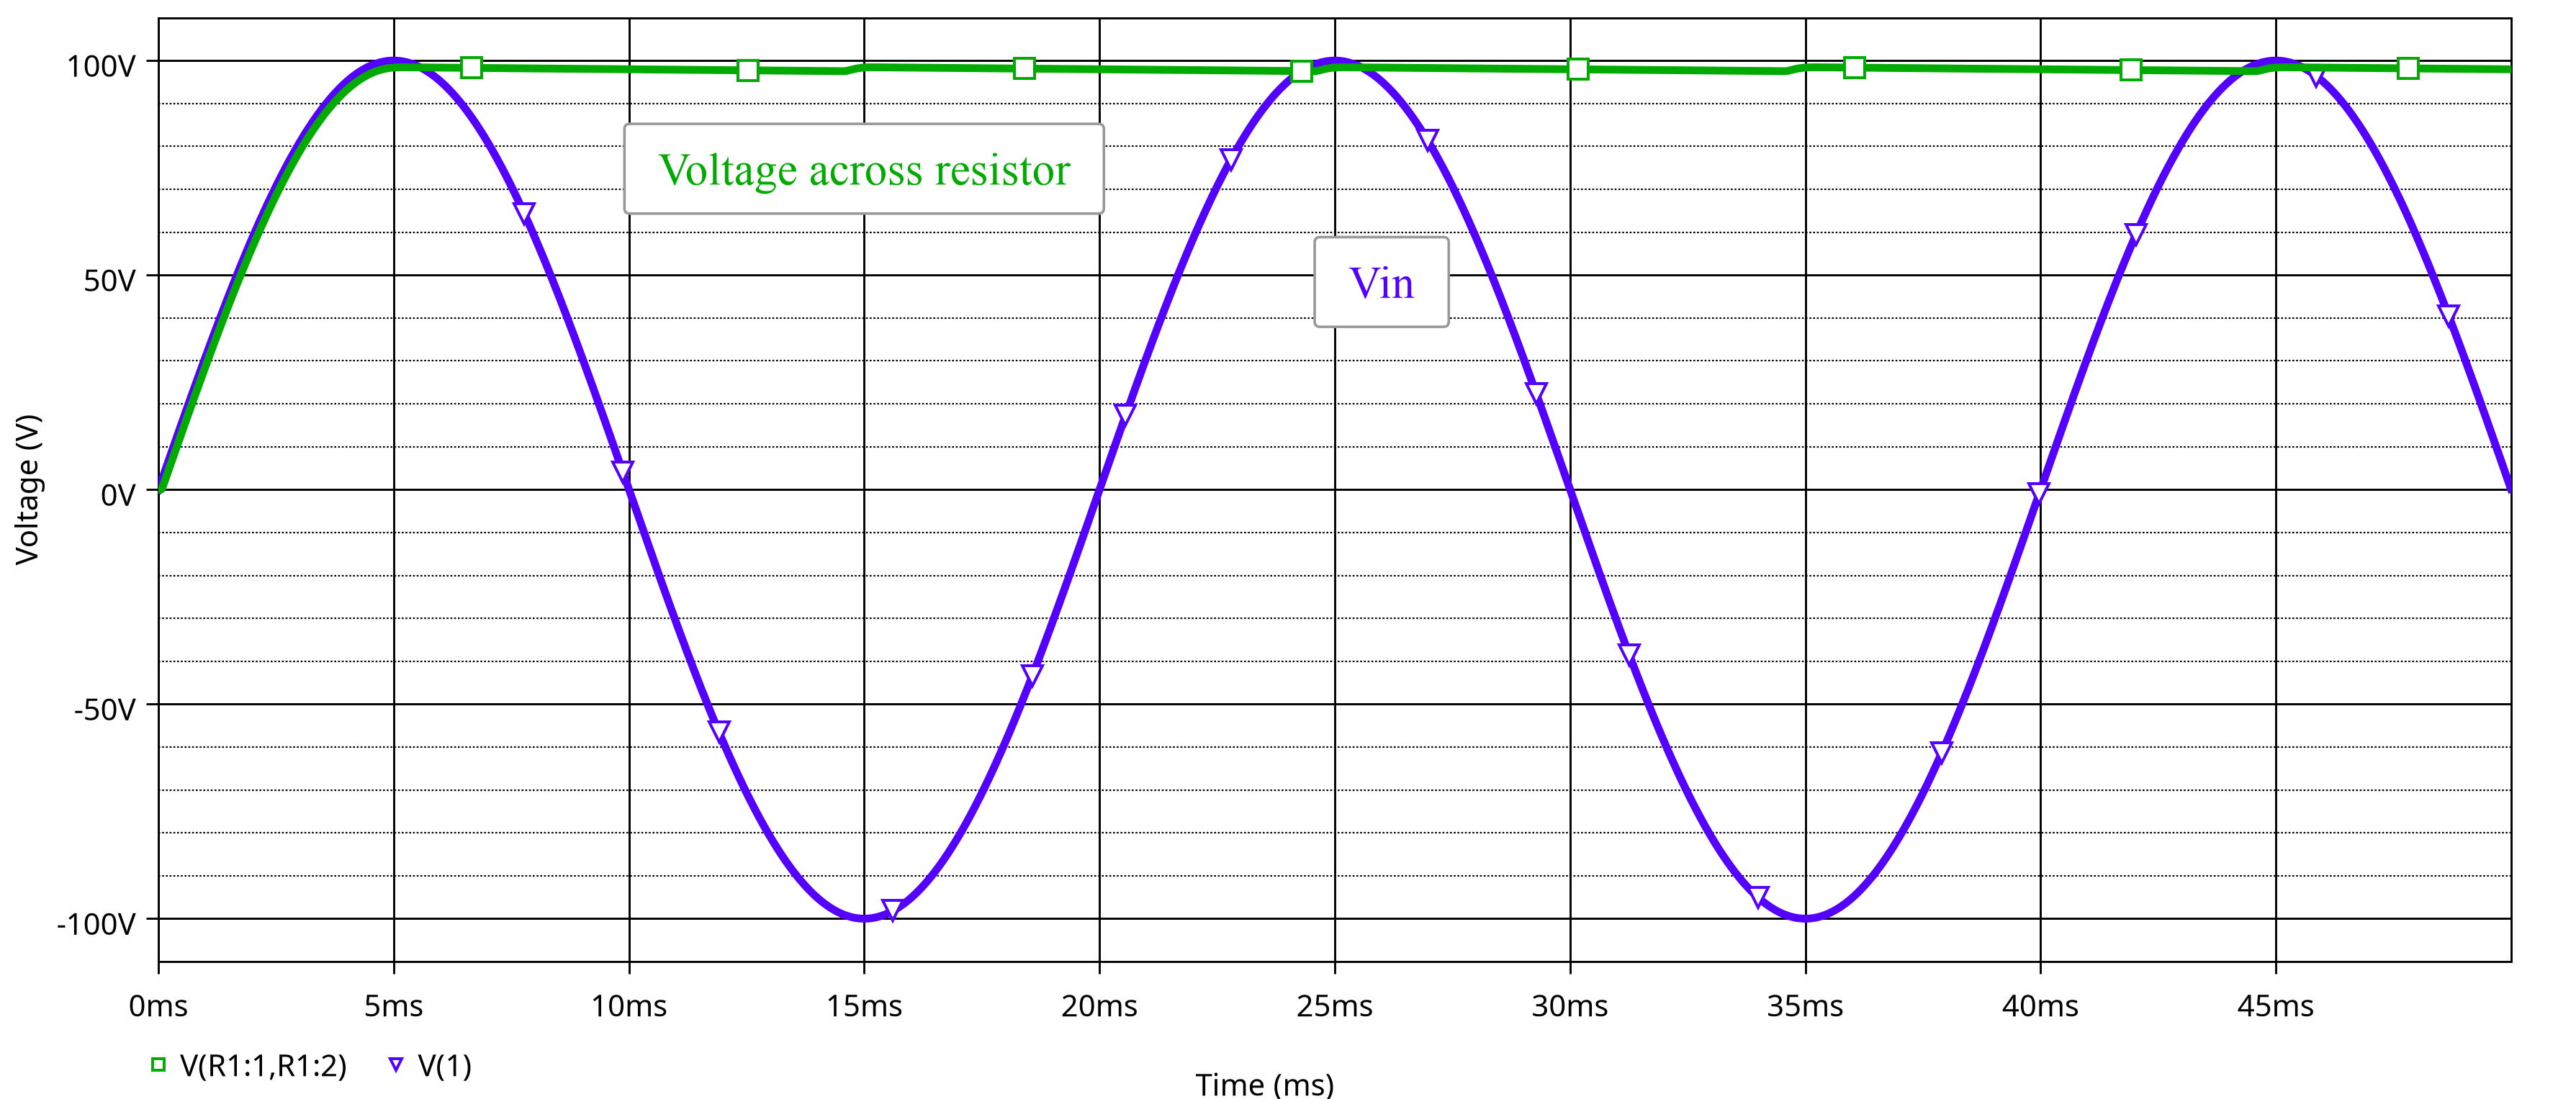
\includegraphics[width=0.8\textwidth]{full_bridge_with_capacitor.png}
		\caption{PSpice output: input and load-voltage waveforms of the
			bridge rectifier with $C_1 = \SI{100}{\micro\farad}$}
		\label{fig:wave2}
	\end{figure}
	
	\begin{figure}[H]
		\centering
		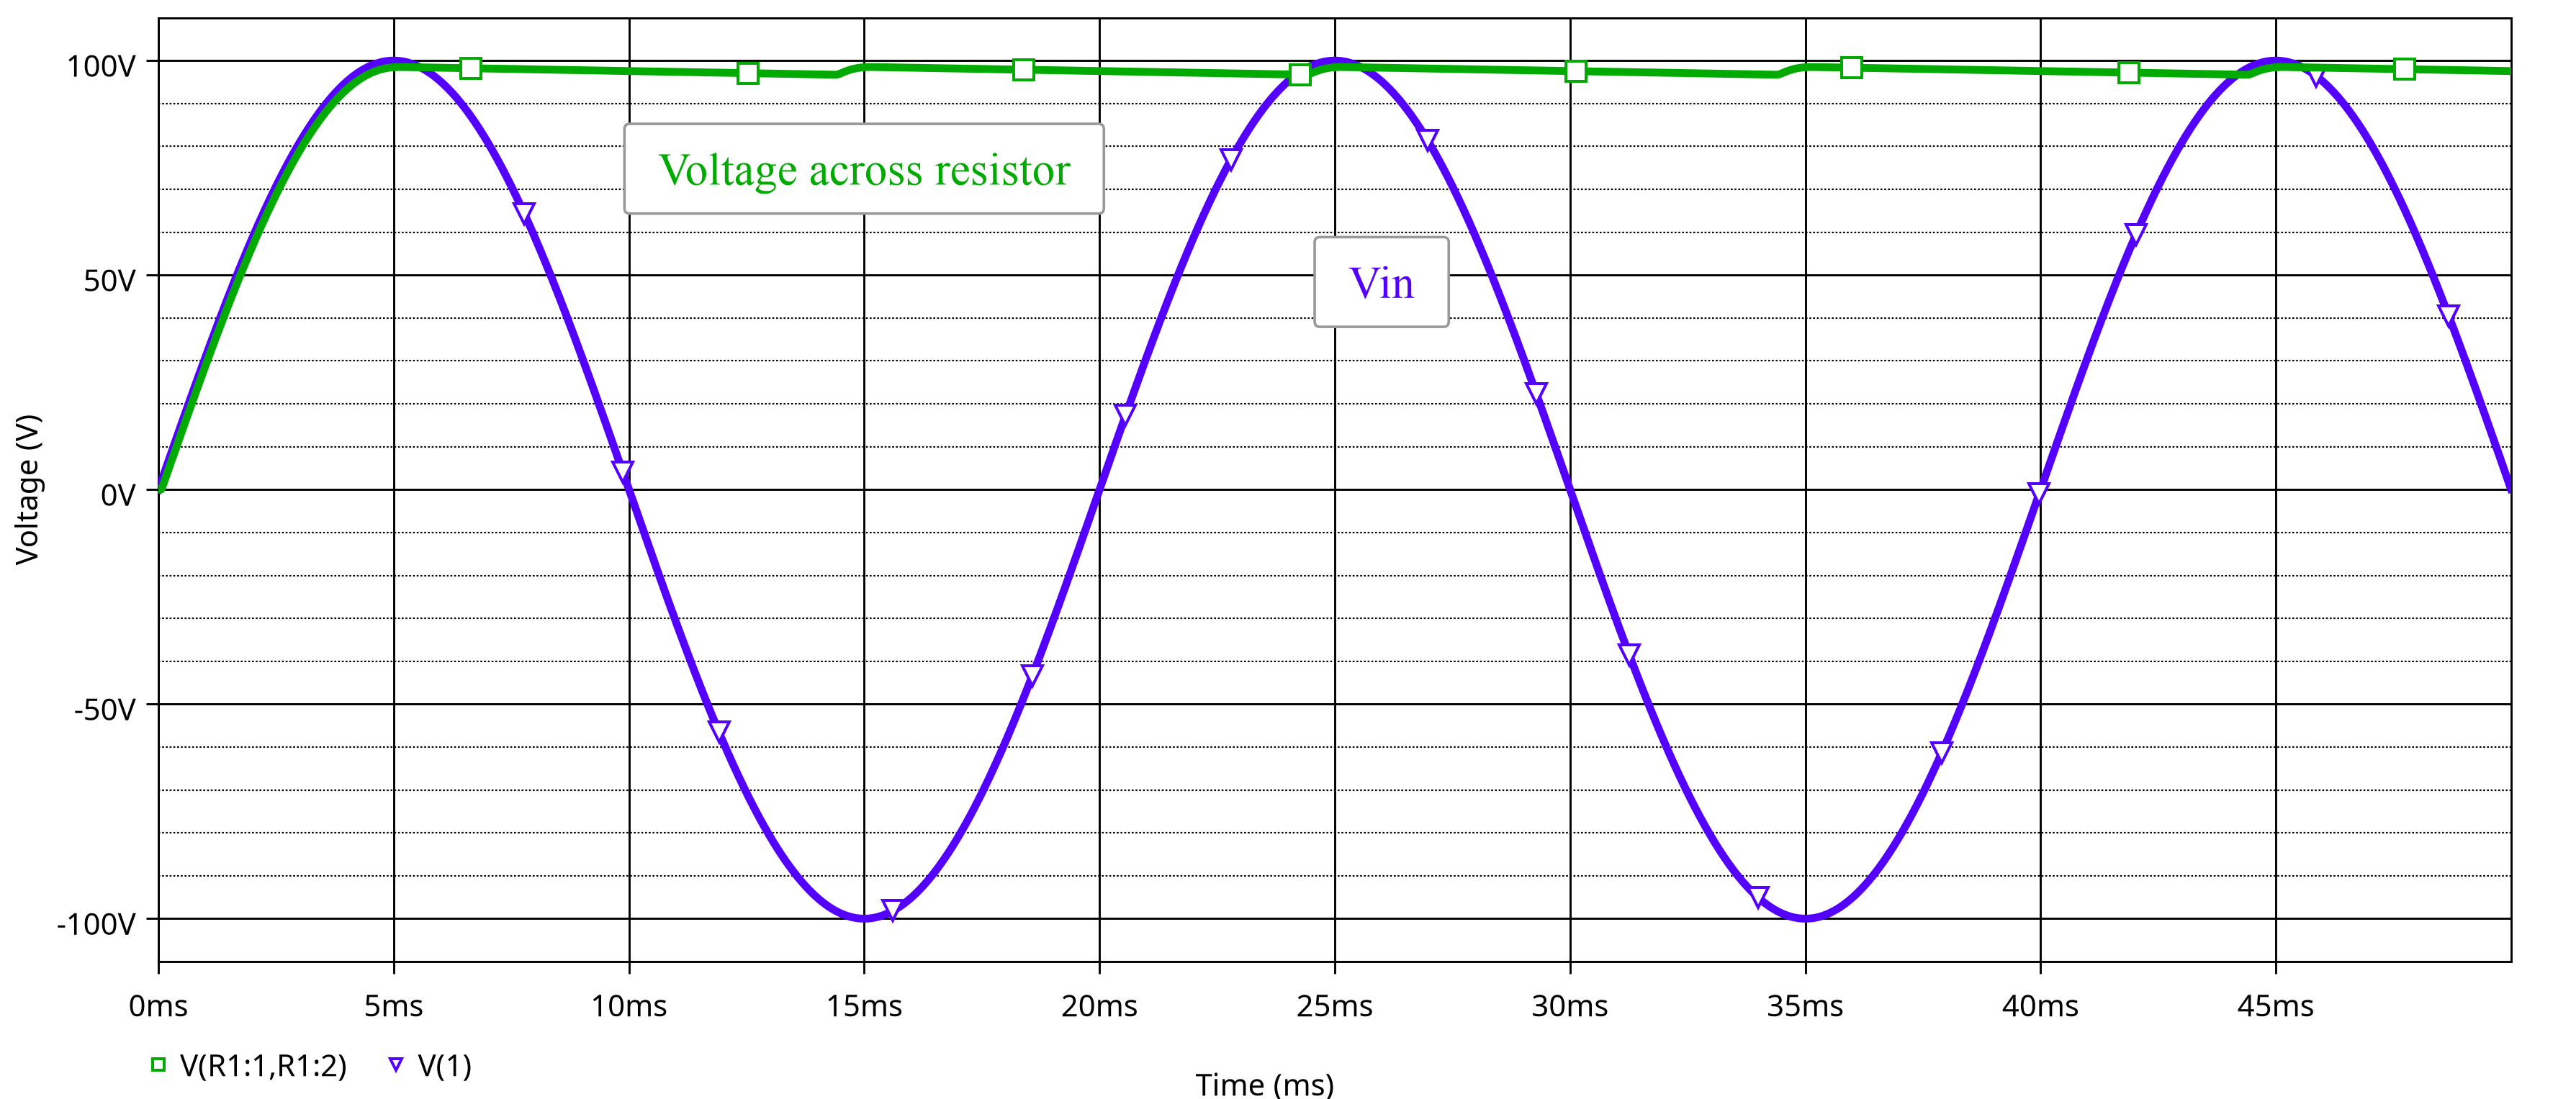
\includegraphics[width=0.8\textwidth]{full_bridge_with_capacitor_changed.png}
		\caption{PSpice output: input and load-voltage waveforms of the
			bridge rectifier with the modified $C_1 = \SI{50}{\micro\farad}$
			(task 4)}
		\label{fig:wave3}
	\end{figure}
	
\end{document}